\section{Exercise 1 - 20-times, Revolutions }
\subsection{Crumbling barricades }
To implemented this the barricade class has to be changed. This class needs to extend the crumbling interface and implements it methods. The UIElementBarricade also needs to be changed to support drawing crumbled barricades. The third and last class that needs to be changed is the Collisions class so the data about the location where a barricade is hit can be used for crumbling the barricade. The collisons class also has to support collisions with partly crumbled barricades.
\newpage
\subsubsection{UML Crumbling barricades}
Figure \ref{fig:1-1barricadeClass} contains the UML class diagram for the crumbling barricades.
To make the working of the crumbling barricade more clear figure Figure \ref{fig:1-1barricadeSequence} contains the sequence diagram concerning the crumbling barricades.
\begin{figure}[ht!]
\centering
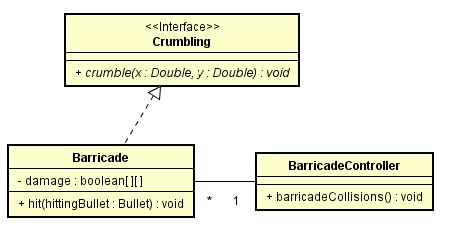
\includegraphics[width=9cm]{BarricadeClass.jpg}
\caption{Barricade UML class Diagram}
\label{fig:1-1barricadeClass}
\end{figure}
\begin{figure}[ht!]
\centering
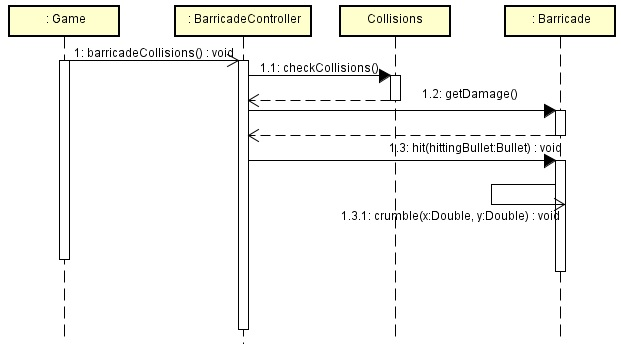
\includegraphics[width=18cm]{BarricadeSequence.jpg}
\caption{Barricade UML class Diagram}
\label{fig:1-1barricadeSequence}
\end{figure}
\newpage
\subsection{ Boss Alien}
\begin{center}
    \begin{tabular}{ | p{4.5cm} | p{3cm} | p{3cm} | p{3cm} | p{1cm} |}
  \hline
    Class & Responsibility & Collaborates with & Super & Sub \\ \hline
   BossAlien & Shooting, movement  &  & Alien & \\ \hline

    \end{tabular}
\end{center}
The game has an integer which remembers in which wave we are so on the n-th wave the special bose wave can be loaded by the wavecontroller. 
A new wave with the bose alien has to be created. The wavepattern reader has to be changed to read a bossalien.

\subsection{ Sound effects}
\begin{center}
    \begin{tabular}{ | p{4.5cm} | p{3cm} | p{3cm} | p{3cm} | p{1cm} |}
  \hline
    Class & Responsibility & Collaborates with & Super & Sub \\ \hline
   SoundController & Playing the sounds  & observable classes that could play sounds  &  & \\ \hline
   SoundLoader & Load the sounds  & SoundController  &  & \\ \hline

    \end{tabular}
\end{center}

The classes which perform actions that are assosiated with sounds has to implement the observable pattern.
The SoundController will implement the observer pattern.
\newpage
\subsubsection{ Sound effects UML}
The UML concerning the sounde effects:
\begin{figure}[ht!]
\centering
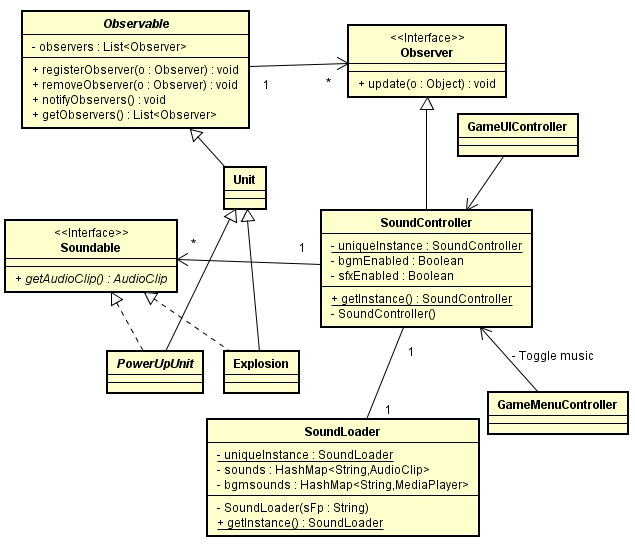
\includegraphics[width=15cm]{sounds.jpg}
\caption{Sounds UML class Diagram}
\label{fig:1-2sounds}
\end{figure}
